\section*{Introduction}

    \begin{figure}[h!]
        \centering
        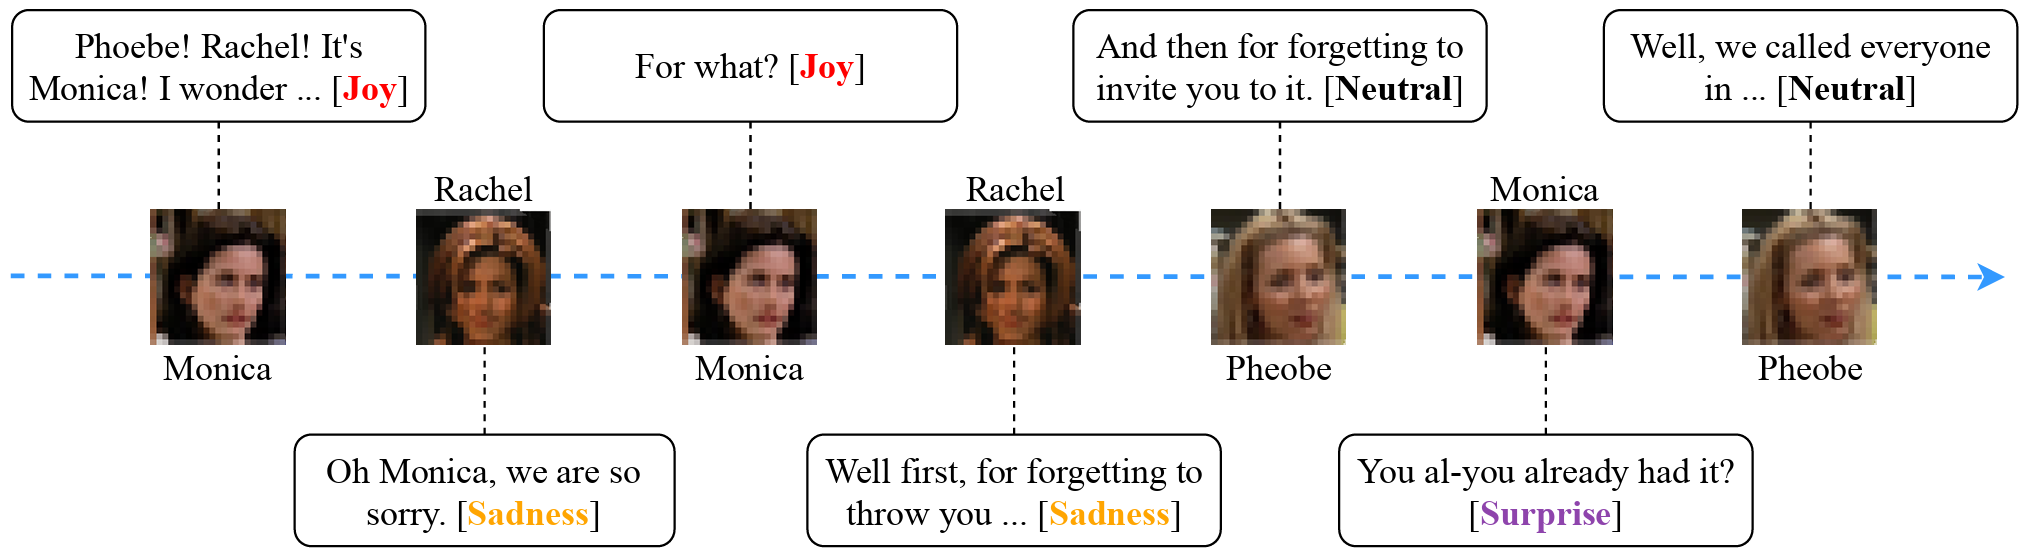
\includegraphics[width=\linewidth]{images/intro_emo.png}
        \captionsetup{width=\linewidth}
        \caption{An example of Emotion Recognition in Conversations. It also depicts  emotional shift of speakers in a dialogue in comparison with their previous emotions. \textit{(Source: \cite{hitrans})}}
        \label{fig:emo}
    \end{figure}



    Humans perceive and understand each other through many channels of communication, whether conveyed through text, audio, or visual cues. Each individual channel has a unique advantage in expressing or communicating the emotional state of a speaker. To understand emotions on a theoretical level, research on emotions has been studied as far back as 1872 \cite{ercontextsota}. Charles Robert Darwin shared his research on the similarity of emotional cues shared by humans and animals in his book "The Expression of the Emotions in Man and Animals." This book concerns the biological aspects of emotional behavior \cite{wikidarwin}. Paul Ekman \cite{ekman}, a psychologist and pioneer in the study of emotions, laid the groundwork by identifying and categorizing universal emotional expressions, illuminating the connection with facial expressions. Ekman identified the six basic emotions as \textit{anger, surprise, disgust, enjoyment, fear,} and \textit{sadness}. Beyond facial expressions, the intonation of sound within speech has emerged as a pivotal aspect of emotion recognition. It refers to the variation of pitch, intensity, and duration of speech sounds. The intonation of sound can convey different emotions, such as happiness, sadness, anger, fear, surprise, and disgust \cite{emocaps}. More recent research has found that small changes in sound can affect human emotions as much as shifts in the tone of a person’s voice \cite{erkin}. This era of increased interactions with devices to perform any task at all has led to the development of an efficient \ac{erc}. Its aim is to identify the emotional states of speakers engaged in dialogue. \ac{erc} has various applications in human-computer interaction, social media analysis, mental health assessment, and affective computing. One of the core aspirations in artificial intelligence is to develop intelligent systems or an empathetic \ac{adh} that can effectively follow multi-modal instructions aligned with human intent to complete various real-world tasks in the wild \cite{visual, assistant}. \ac{erc} is an increasingly popular and challenging task in NLP that aims to identify the emotional state of speakers engaged in dialogue and hence pave a way to create an \ac{adh}. Recent works on \ac{erc} present several solutions with multi-modal datasets and challenges such as conversational context modeling, emotional shifts of the interlocutors, and others. In this survey, we review the recent advances in \ac{erc} methods, focusing on the multi-modal approaches that leverage different sources of information, such as text, audio, and visual cues. We categorize the existing methods into two types: RNN-based, and transformer-based methods. We discuss the advantages and disadvantages of each type and compare their performance on several benchmark datasets. We also present the main challenges and open issues in ERC and suggest some possible directions for future research. The methods we cover in this survey are: CMN, DialogueRNN, DialogueTRM, DialogXL, EmoBERTa, Hi-Trans, M2FNet, FacialMMT, and MultiEMO. These methods are selected based on their novelty, popularity, and effectiveness in ERC. We provide a brief overview of each method and highlight their key contributions and limitations. We also provide a table that summarizes the main characteristics and results of each method.